% Options for packages loaded elsewhere
\PassOptionsToPackage{unicode}{hyperref}
\PassOptionsToPackage{hyphens}{url}
\PassOptionsToPackage{dvipsnames,svgnames,x11names}{xcolor}
%
\documentclass[
  letterpaper,
  DIV=11,
  numbers=noendperiod,
  oneside]{scrartcl}

\usepackage{amsmath,amssymb}
\usepackage{iftex}
\ifPDFTeX
  \usepackage[T1]{fontenc}
  \usepackage[utf8]{inputenc}
  \usepackage{textcomp} % provide euro and other symbols
\else % if luatex or xetex
  \usepackage{unicode-math}
  \defaultfontfeatures{Scale=MatchLowercase}
  \defaultfontfeatures[\rmfamily]{Ligatures=TeX,Scale=1}
\fi
\usepackage{lmodern}
\ifPDFTeX\else  
    % xetex/luatex font selection
\fi
% Use upquote if available, for straight quotes in verbatim environments
\IfFileExists{upquote.sty}{\usepackage{upquote}}{}
\IfFileExists{microtype.sty}{% use microtype if available
  \usepackage[]{microtype}
  \UseMicrotypeSet[protrusion]{basicmath} % disable protrusion for tt fonts
}{}
\makeatletter
\@ifundefined{KOMAClassName}{% if non-KOMA class
  \IfFileExists{parskip.sty}{%
    \usepackage{parskip}
  }{% else
    \setlength{\parindent}{0pt}
    \setlength{\parskip}{6pt plus 2pt minus 1pt}}
}{% if KOMA class
  \KOMAoptions{parskip=half}}
\makeatother
\usepackage{xcolor}
\usepackage[left=1in,marginparwidth=2.0666666666667in,textwidth=4.1333333333333in,marginparsep=0.3in]{geometry}
\ifLuaTeX
  \usepackage{luacolor}
  \usepackage[soul]{lua-ul}
\else
  \usepackage{soul}
  
\fi
\setlength{\emergencystretch}{3em} % prevent overfull lines
\setcounter{secnumdepth}{-\maxdimen} % remove section numbering
% Make \paragraph and \subparagraph free-standing
\ifx\paragraph\undefined\else
  \let\oldparagraph\paragraph
  \renewcommand{\paragraph}[1]{\oldparagraph{#1}\mbox{}}
\fi
\ifx\subparagraph\undefined\else
  \let\oldsubparagraph\subparagraph
  \renewcommand{\subparagraph}[1]{\oldsubparagraph{#1}\mbox{}}
\fi


\providecommand{\tightlist}{%
  \setlength{\itemsep}{0pt}\setlength{\parskip}{0pt}}\usepackage{longtable,booktabs,array}
\usepackage{calc} % for calculating minipage widths
% Correct order of tables after \paragraph or \subparagraph
\usepackage{etoolbox}
\makeatletter
\patchcmd\longtable{\par}{\if@noskipsec\mbox{}\fi\par}{}{}
\makeatother
% Allow footnotes in longtable head/foot
\IfFileExists{footnotehyper.sty}{\usepackage{footnotehyper}}{\usepackage{footnote}}
\makesavenoteenv{longtable}
\usepackage{graphicx}
\makeatletter
\def\maxwidth{\ifdim\Gin@nat@width>\linewidth\linewidth\else\Gin@nat@width\fi}
\def\maxheight{\ifdim\Gin@nat@height>\textheight\textheight\else\Gin@nat@height\fi}
\makeatother
% Scale images if necessary, so that they will not overflow the page
% margins by default, and it is still possible to overwrite the defaults
% using explicit options in \includegraphics[width, height, ...]{}
\setkeys{Gin}{width=\maxwidth,height=\maxheight,keepaspectratio}
% Set default figure placement to htbp
\makeatletter
\def\fps@figure{htbp}
\makeatother
% definitions for citeproc citations
\NewDocumentCommand\citeproctext{}{}
\NewDocumentCommand\citeproc{mm}{%
  \begingroup\def\citeproctext{#2}\cite{#1}\endgroup}
\makeatletter
 % allow citations to break across lines
 \let\@cite@ofmt\@firstofone
 % avoid brackets around text for \cite:
 \def\@biblabel#1{}
 \def\@cite#1#2{{#1\if@tempswa , #2\fi}}
\makeatother
\newlength{\cslhangindent}
\setlength{\cslhangindent}{1.5em}
\newlength{\csllabelwidth}
\setlength{\csllabelwidth}{3em}
\newenvironment{CSLReferences}[2] % #1 hanging-indent, #2 entry-spacing
 {\begin{list}{}{%
  \setlength{\itemindent}{0pt}
  \setlength{\leftmargin}{0pt}
  \setlength{\parsep}{0pt}
  % turn on hanging indent if param 1 is 1
  \ifodd #1
   \setlength{\leftmargin}{\cslhangindent}
   \setlength{\itemindent}{-1\cslhangindent}
  \fi
  % set entry spacing
  \setlength{\itemsep}{#2\baselineskip}}}
 {\end{list}}
\usepackage{calc}
\newcommand{\CSLBlock}[1]{\hfill\break\parbox[t]{\linewidth}{\strut\ignorespaces#1\strut}}
\newcommand{\CSLLeftMargin}[1]{\parbox[t]{\csllabelwidth}{\strut#1\strut}}
\newcommand{\CSLRightInline}[1]{\parbox[t]{\linewidth - \csllabelwidth}{\strut#1\strut}}
\newcommand{\CSLIndent}[1]{\hspace{\cslhangindent}#1}

\KOMAoption{captions}{tableheading}
\makeatletter
\@ifpackageloaded{caption}{}{\usepackage{caption}}
\AtBeginDocument{%
\ifdefined\contentsname
  \renewcommand*\contentsname{Table of contents}
\else
  \newcommand\contentsname{Table of contents}
\fi
\ifdefined\listfigurename
  \renewcommand*\listfigurename{List of Figures}
\else
  \newcommand\listfigurename{List of Figures}
\fi
\ifdefined\listtablename
  \renewcommand*\listtablename{List of Tables}
\else
  \newcommand\listtablename{List of Tables}
\fi
\ifdefined\figurename
  \renewcommand*\figurename{Figure}
\else
  \newcommand\figurename{Figure}
\fi
\ifdefined\tablename
  \renewcommand*\tablename{Table}
\else
  \newcommand\tablename{Table}
\fi
}
\@ifpackageloaded{float}{}{\usepackage{float}}
\floatstyle{ruled}
\@ifundefined{c@chapter}{\newfloat{codelisting}{h}{lop}}{\newfloat{codelisting}{h}{lop}[chapter]}
\floatname{codelisting}{Listing}
\newcommand*\listoflistings{\listof{codelisting}{List of Listings}}
\makeatother
\makeatletter
\makeatother
\makeatletter
\@ifpackageloaded{caption}{}{\usepackage{caption}}
\@ifpackageloaded{subcaption}{}{\usepackage{subcaption}}
\makeatother
\makeatletter
\@ifpackageloaded{sidenotes}{}{\usepackage{sidenotes}}
\@ifpackageloaded{marginnote}{}{\usepackage{marginnote}}
\makeatother
\ifLuaTeX
  \usepackage{selnolig}  % disable illegal ligatures
\fi
\usepackage{bookmark}

\IfFileExists{xurl.sty}{\usepackage{xurl}}{} % add URL line breaks if available
\urlstyle{same} % disable monospaced font for URLs
\hypersetup{
  pdftitle={Manuscript 1},
  pdfauthor={Andreas Ludvig Ohm Svendsen; Tore B. Stage},
  pdfkeywords={3D primary human hepatocytes, Inflammation, Drug
metabolism},
  colorlinks=true,
  linkcolor={blue},
  filecolor={Maroon},
  citecolor={Blue},
  urlcolor={Blue},
  pdfcreator={LaTeX via pandoc}}

\title{Manuscript 1}
\author{Andreas Ludvig Ohm Svendsen \and Tore B. Stage}
\date{2024-01-26}

\begin{document}
\maketitle
\begin{abstract}
This is an abstract \ldots{}
\end{abstract}

\subsection{Introduction}\label{introduction}

Inflammation is a complex biological response that is pivotal in various
pathological conditions. These range from systemic inflammatory
diseases, such as rheumatoid arthritis and sepsis, to lower-grade
chronic inflammatory states such as type 2 diabetes mellitus. Given the
prevalence of systemic inflammation, understanding its interaction with
drug metabolism is of substantial clinical relevance.

Drug-metabolizing enzymes and transporters (DMETs), predominantly found
in hepatocytes within the liver, are central to the biotransformation of
a wide variety of compounds. Inflammation has been shown to modulate the
activity of these DMETs, a phenomenon that could potentially affect the
pharmacokinetics of numerous medications. For individuals with altered
inflammatory status---whether due to a chronic condition like diabetes
or an acute event like sepsis---this modulation can have significant
implications. It may necessitate adjustments in drug dosages to avoid
adverse effects or therapeutic failure.

Previous research has provided valuable insights into the effects of
inflammation on DMETs, but a clear correlation between in vitro studies
and clinical observations remains elusive. For instance Dunvald et al.
(1) conducted a comprehensive review of the clinical and in vitro
evidence on inflammation-mediated modulation of DMETs and the impact on
drug metabolism in humans. They found that in vitro studies in primary
human hepatocytes revealed strong evidence of downregulation of key
cytochrome P450 (CYP) enzymes by inflammatory cytokines such as IL-6 and
IL-1β. However, these studies often employed supraphysiological cytokine
doses, which may not accurately represent the inflammatory conditions
observed in patients.

Levels of IL-6 and IL-1B in healthy individuals are generally low, with
reports in range of \textasciitilde10pg/ml in adults for IL-6, and
\textasciitilde2.5 pg/ml IL-1B in adults (2--5). In contrast, cytokine
levels may be considerably elevated with IL-6 levels of
\textasciitilde140 pg/mL, and I\ul{L-1B levels of \textasciitilde100
pg/mL}, among patients with rheumatoid arthritis or SLE (6) to more than
1 ng/mL of IL-6 for patients with acute inflammation caused by sepsis
(7). These variations in cytokine levels, which span a wide range in
different pathological states, highlight the complex and dynamic nature
of inflammation and underscore the need for research that considers this
variability when investigating the effects of inflammation on
drug-metabolizing enzymes.

Recently, 3D primary human hepatocytes (PHH) have challenged 2D PHH as a
more physiologically relevant culture method of PHH. 3D culture leads to
more stable cell cultures that retain their hepatic phenotype for
extended periods of time (8). Consequently, this 3D PHH have been shown
to predict CYP induction and hepatotoxicity more accurately than 2D PHH
(9,10). Historically, 2D PHH have been utilized to study the effect of
drugs and inflammation on hepatocyte/liver function. However, the
inherent limitations of 2D cultures, primarily their inability to
maintain the physiological phenotype and liver-specific functions of
hepatocytes, have prompted a shift towards the 3D liver spheroid models.
This model is increasingly recognized for their physiological relevance
and stability, offering a more accurate representation of hepatic
responses. The 3D liver spheroids preserve liver cell phenotypes and
functions over extended periods, thereby enhancing the reliability of
drug-induced liver injury predictions and disease mechanism
investigations. This advancement positions 3D liver spheroids as
potentially the new standard for in vitro hepatocyte studies, while
still being suitable for a high throughput setting, and financially
accessible as opposed to even more advanced liver models (ref for last
part) (1,11) . Another claim for the lack of correlation discussed in
the review by AC et al.~is that there might be methodological
limitations to the widespread use of 2D models of PHHs (1).

We aimed to utilize 3D primary human hepatocytes (8) to study the impact
of physiologically relevant concentrations of cytokines on CYP
expression and activity. This may help further our understanding of the
impact of inflammation on clinical drug metabolism among patients with
inflammation. This, in turn, may inform more precise and adaptive
prescribing strategies for patients in various inflammatory states.

\subsection{Methods}\label{methods}

\subsubsection{3D spheroid culture of
PHHs}\label{d-spheroid-culture-of-phhs}

\paragraph{Materials}\label{materials}

All necessary components for cell culture, including the medium,
supplements, and compounds, were acquired from Thermo Fisher Scientific,
unless stated otherwise.

\paragraph{Cell source and
preparation}\label{cell-source-and-preparation}

Three lots of cryopreserved primary human hepatocytes, specifically
Hu8345-A, Hu8373-A and Hu8381, were procured from Thermo Fisher
Scientific (Waltham, MA). All necessary cell culture reagents were
sourced from the same supplier. All PHHs were qualified for spheroid
formation per the manufacturer.

\paragraph{Spheroid formation and
maintenance}\label{spheroid-formation-and-maintenance}

The spheroid culture followed an adapted protocol from a previous study
(8). In short 1500 hepatocytes per well in ultra-low attachment 96-well
plates. Following seeding, the plates were centrifuged for 2 minutes at
200g. Subsequently, the plates were incubated at 37°C with 5\% CO2.

On day 0 cells were seeded in culture medium, totaling 100 μL per well,
consisting of 5\% fetal bovine serum, 1 μM dexamethasone, 5 μg/mL human
recombinant insulin, 100 U/mL penicillin, 100 μg/mL streptomycin, 2 mM
L-glutamine, and 15 mM HEPES in Williams' E medium.

After spheroid formation the seeding medium was replaced with FBS free
maintenance medium. This medium comprised 0.1 μM dexamethasone, 10 μg/mL
human recombinant insulin, 5.5 μg/mL transferrin, 6.7 ng/mL selenium,
100 U/mL penicillin, 100 μg/mL streptomycin, and 2 mM L-glutamine in
Williams' E medium. This FBS washout with maintenance medium was done
with a 70\% medium change on days 5-7.
\texttt{For\ donor\ 1\ (Hu8345-A)\ the\ maintenance\ also\ contained\ 5.35 μg/mL\ linoleic\ acid,\ 1.25 mg/mL\ bovine\ serum\ albumin\ and\ 15 mM\ HEPES.\ These\ supplements\ are,\ however,\ no\ longer\ recommended\ by\ the\ manufacturer}\sidenote{\footnotesize Skip
  this?}\texttt{.}

Detailed descriptions of the spheroid culture process, as well as donor
information, are available in the supplementary materials (Table SX).

\subsubsection{Treatments}\label{treatments}

Treatment with proinflammatory cytokines commenced on day 8 post
seeding. The spheroids were exposed to IL-6 and IL-1β at concentrations
of 0.01, 0.1, 1, and 10 ng/ml, alongside a vehicle control (0.1\% bovine
serum albumin in PBS). The cytokine treatments and vehicle control were
diluted 1:1000 in the culture medium before administration.Re-dosing was
done every other day for long-term cultures.

\subsubsection{Spheroid viability and
morphology}\label{spheroid-viability-and-morphology}

The viability of the spheroids was monitored by measuring their ATP
content, using the luminiscence CellTiter-Glo 3D assay from Promega
(Madison, WI). Quantification of ATP was done using an ATP (from Thermo
Fisher Scientific) standard curve. Viability was assessed every 2-3 days
throughout the experiments.

In addition to viability testing, the morphology of the spheroids was
monitored. Imaging was done every second or third day, aligning with the
viability assays. The spheroids were imaged using a light microscope
equipped with a 10X magnification lens and a digital camera from Motic
(Hong Kong, China).

\subsubsection{RNA extraction, cDNA synthesis and
qPCR}\label{rna-extraction-cdna-synthesis-and-qpcr}

RNA was extracted using the phenol-chloroform method, following the
manufacturer's protocol from Qiagen with minor modifications (12). Each
spheroid pool was treated with 1 mL of Qiazol (Qiagen) reagent for
lysis, followed by co-precipitation with 15 μg of RNA grade glycogen
(Thermo Fisher Scientific). The RNA pellet underwent three washes with
75\% ethanol. Post-wash, a combination of heating and evaporation
techniques was applied to remove residual ethanol and to facilitate the
solubilization of the RNA pellet in water.

RNA integrity was assessed for a subset of samples\sidenote{\footnotesize Dog ikke fra
  nogle af disse 3 donorer, så måske bedre med: To assess the integrity
  of the RNA, we evaluated the RNA Integrity Number (RIN) for a subset
  of samples, which yielded values ranging from 7 to 9.8.\\
  \strut \\
  To validate the RNA extraction method, we assessed the RNA Integrity
  Number (RIN) using the Agilent BioAnalyzer for a subset of samples not
  derived from the donors discussed in this article. These assessments
  yielded RIN values between 7 and 9.8, indicative of high-quality RNA.}
using the Agilent BioAnalyzer, yielding RNA Integrity Number (RIN)
values from 7 to 9.8. These values indicate high-quality RNA.
Concentration of RNA were estimated utilizing the NanoDrop
spectrophotometer.

Approximately 500 ng of extracted RNA was used for cDNA synthesis. This
process was performed using the High-Capacity cDNA Reverse Transcription
Kit with RNase Inhibitor (Thermo Fisher Scientific).

For qPCR, 10 ng of cDNA, based on the initial RNA concentration, was
utilized for each reaction. The reactions were set up in a 10 μL volume
containing TaqMan Universal Master Mix II and target-specific TaqMan
assays (detailed in Supplementary Methods). The qPCR was run for 40
cycles, following the manufacturer's guidelines (Thermo Fisher
Scientific). The PCR plate sample maximization method was applied(13),
and a stable reference gene as well as no template controls and no
reverse transcriptase controls was included in each plate.

In the analysis of mRNA expression, the relative quantity was calculated
by first determining the delta Cq ((\Delta C\_q)) for each sample. This
was achieved by subtracting the mean Cq of the control group from the
mean Cq of the replicates of each sample. The relative quantity was then
computed using the formula (2\^{}\{\Delta C\_q\}). For normalization,
the relative quantity of the target gene in each sample was divided by
the relative quantity of the reference gene (GAPDH or TBP). The average
normalized expression for each biological group was subsequently
calculated.

\subsubsection{Activity}\label{activity}

To assess the activity of CYP3A4 (maybe otheres also), an experiment was
conducted using midazolam as a substrate in spheroids derived from
donors 2 and 3, evaluated on day 12. Midazolam (Toronto Research
Chemicals, Toronto, ON, Canada), was prepared as a 6,000× stock solution
in DMSO. The final DMSO concentration in the enzyme activity assays was
maintained at 0.15\%. Prior to the introduction of midazolam to the
spheroids, the cells underwent three washes with 100 μL of maintenance
medium. Between washes, the residual volume was kept at 20 μL, and
before the final wash, the spheroids were incubated for 2 hours in a
cell culture incubator.

The concentration of midazolam in the assay was set at 10 μM, with a
total volume of 100 μL per well. For the analysis, triplicate samples,
each comprising a \st{spheroid} and medium from a single well, were
collected at 0.5 (8 hours for other enzymes) hours post midazolam
treatment. These samples were then stored at -80°C until further
analysis. The specific methods used for the metabolite analysis of these
samples are detailed in the supplementary material.

\subsubsection{Quantitative analysis of proteins via LC-MS with
selective
immunoprecipitation}\label{quantitative-analysis-of-proteins-via-lc-ms-with-selective-immunoprecipitation}

The quantification of human CYP \st{and transporter} proteins was
performed using a targeted liquid chromatography-mass spectrometry
approach, incorporating selective immunoprecipitation of peptides, as
previously described(14). Uniform numbers of spheroids were employed in
each analysis for consistency. In summary, spheroids were lysed in a
buffer of 42 mM ammonium bicarbonate, containing 1.14 mM dithiothreitol
and 9 mM iodoacetamide, and incubated for 15 minutes at 90°C, a method
adapted from Savaryn et al. (15). The lysates were then digested with
MS-grade Pierce Trypsin Protease (Thermo Fisher Scientific) for 16 hours
at 37°C. To halt the digestion, phenylmethanesulfonyl fluoride was added
to each sample, achieving a final concentration of 1 mM and a total
volume of 70 μL. A portion of the digested sample (25 μL) was then used
for the immunoprecipitation of surrogate and internal standard peptides
using triple X proteomics antibodies(14). These peptides were
subsequently analyzed and quantified through LC-MS. The specific
surrogate peptides employed for protein quantification and the
LC-gradients are detailed in the supplementary material. For data
processing, Skyline software (MACOSS Lab, University of Washington,
Seattle, WA) and TraceFinder 4.1 (Thermo Fisher Scientific) were
utilized.

\subsection{Results}\label{results}

\subsubsection{Viability and morphology}\label{viability-and-morphology}

Mean relative viability is seen in
Figure~\ref{fig-viability-relative-overall}.

\begin{figure}[H]

\centering{

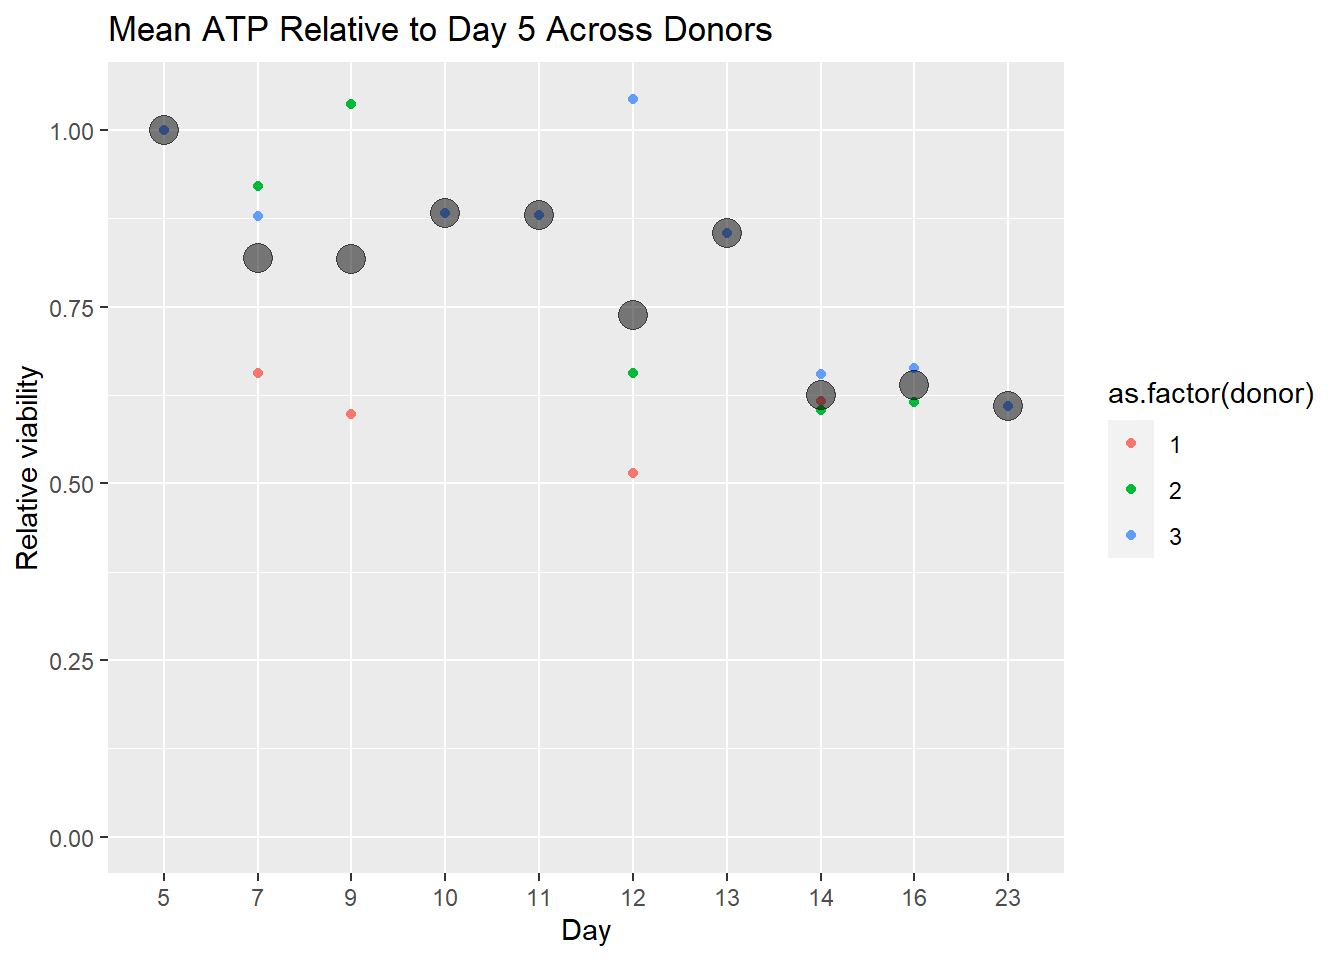
\includegraphics{index_files/figure-latex/notebooks-viability-Viability-fig-viability-relative-overall-output-1.png}

}

\caption{\label{fig-viability-relative-overall}Note that the
concentration of ATP of donor one on day 5 was to high. Data for this
donor/day not trustworthy/viability to high. This yields a steep fall
from day 5 to 7}

\end{figure}%

\textsubscript{Source:
\href{https://andreasludvig.github.io/manuscript_one/notebooks/viability/Viability-preview.html\#cell-fig-viability-relative-overall}{Viability}}

The individual viability for each donor is seen in
Figure~\ref{fig-donor-viabilities}. This fig is inserted as an image.

\begin{figure}[H]

\centering{

\captionsetup{labelsep=none}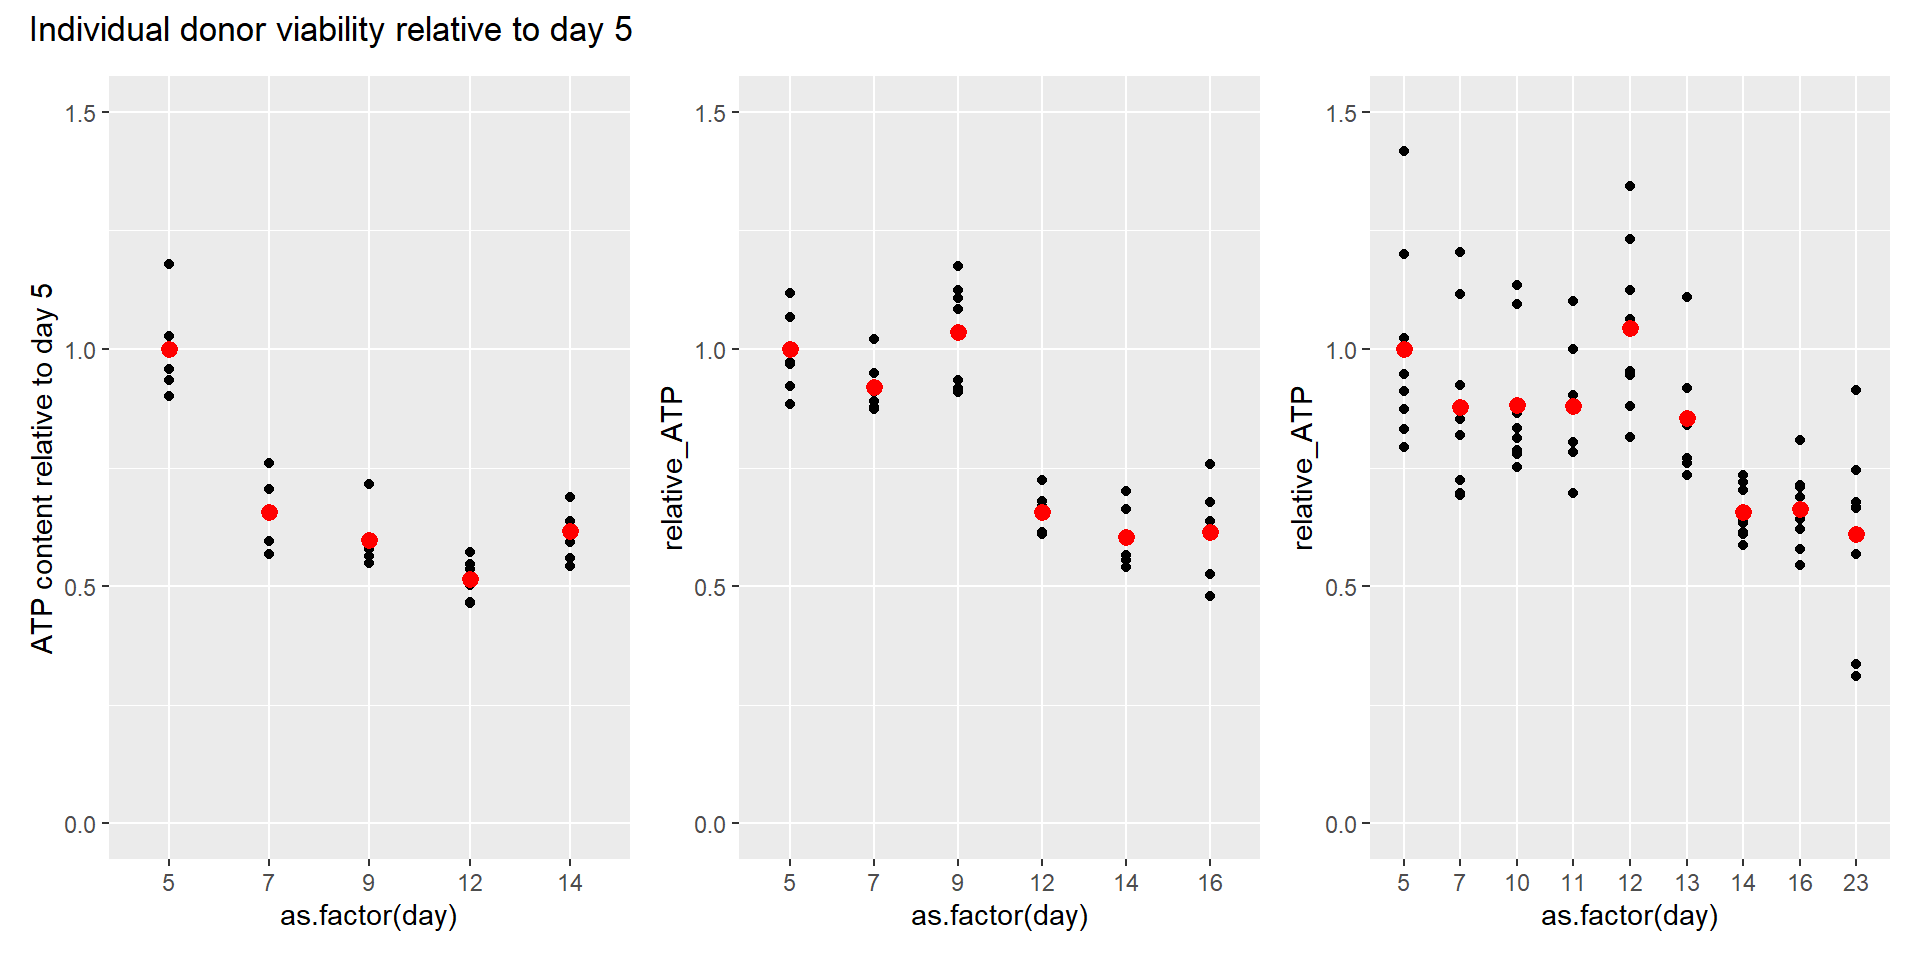
\includegraphics{index_files/figure-latex/notebooks-viability-Viability-fig-donor-viabilities-output-2.png}

}

\caption{\label{fig-donor-viabilities}}

\end{figure}%

\textsubscript{Source:
\href{https://andreasludvig.github.io/manuscript_one/notebooks/viability/Viability-preview.html\#cell-fig-donor-viabilities}{Viability}}

Absolute overall viability is seen in
Figure~\ref{fig-viability-absolute-overall}

\begin{figure}[H]

\centering{

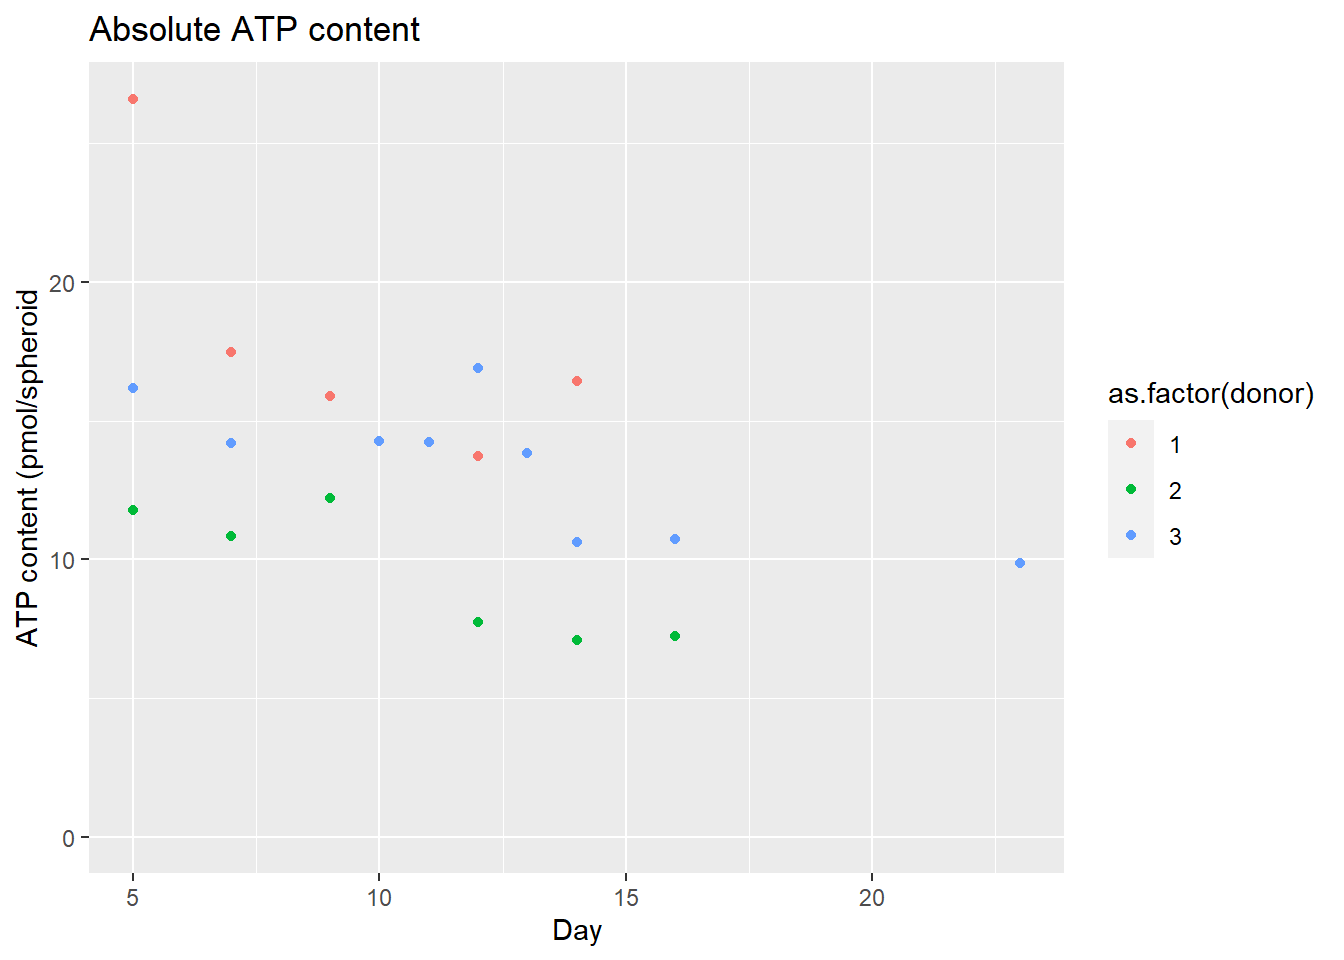
\includegraphics{index_files/figure-latex/notebooks-viability-Viability-fig-viability-absolute-overall-output-1.png}

}

\caption{\label{fig-viability-absolute-overall}Note that the
concentration of ATP of donor one on day 5 was to high. Data for this
donor/day not trustworthy/viability to high}

\end{figure}%

\textsubscript{Source:
\href{https://andreasludvig.github.io/manuscript_one/notebooks/viability/Viability-preview.html\#cell-fig-viability-absolute-overall}{Viability}}

Morphology of the spheroids over time is seen in Figure~\ref{fig-morph}

\begin{figure}

\centering{

\captionsetup{labelsep=none}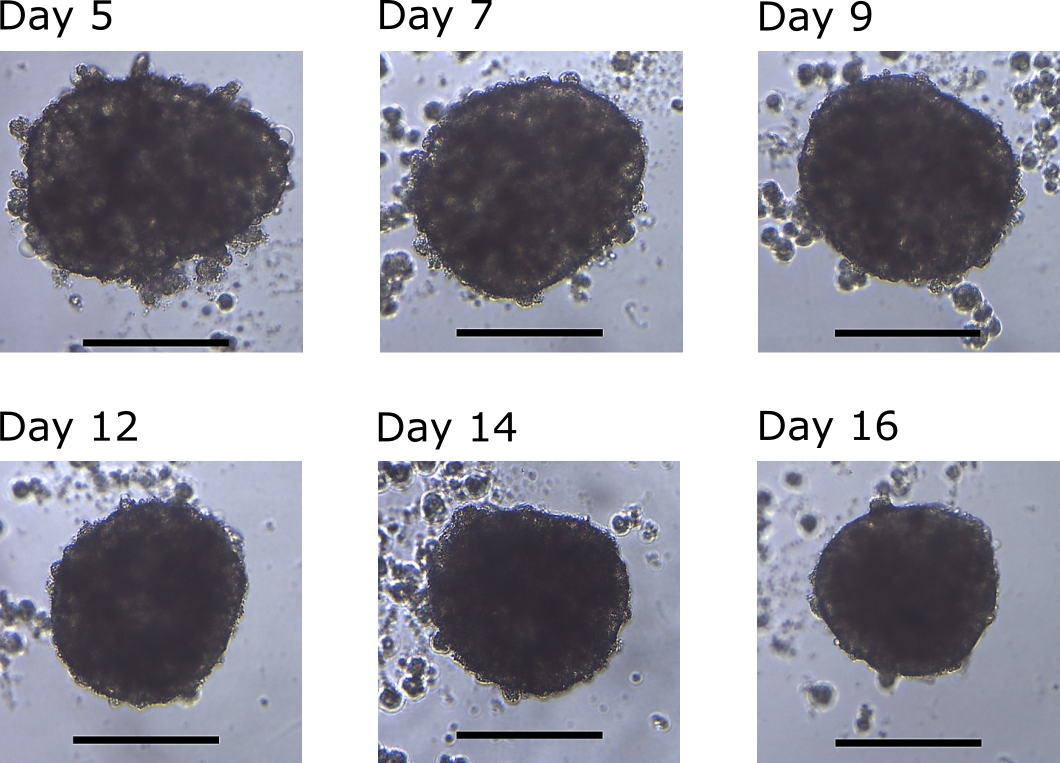
\includegraphics{images/morphology_AS0006.png}

}

\caption{\label{fig-morph}}

\end{figure}%

\subsubsection{mRNA}\label{mrna}

\subsubsection{Activity}\label{activity-1}

\subsection*{References}\label{references}
\addcontentsline{toc}{subsection}{References}

\phantomsection\label{refs}
\begin{CSLReferences}{0}{1}
\bibitem[\citeproctext]{ref-dunvald}
\CSLLeftMargin{1. }%
\CSLRightInline{Dunvald ACD, Järvinen E, Mortensen C, Stage TB. Clinical
and Molecular Perspectives on Inflammation-Mediated Regulation of Drug
Metabolism and Transport. Clinical Pharmacology \& Therapeutics
{[}Internet{]}. n/a(n/a). Available from:
\url{https://onlinelibrary.wiley.com/doi/abs/10.1002/cpt.2432}}

\bibitem[\citeproctext]{ref-kim2011}
\CSLLeftMargin{2. }%
\CSLRightInline{Kim HO, Kim HS, Youn JC, Shin EC, Park S. Serum cytokine
profiles in healthy young and elderly population assessed using
multiplexed bead-based immunoassays. Journal of Translational Medicine
{[}Internet{]}. 2011 Jul 20;9(1):113. Available from:
\url{https://doi.org/10.1186/1479-5876-9-113}}

\bibitem[\citeproctext]{ref-kleiner2013}
\CSLLeftMargin{3. }%
\CSLRightInline{Kleiner G, Marcuzzi A, Zanin V, Monasta L, Zauli G.
Cytokine Levels in the Serum of Healthy Subjects. Mediators of
Inflammation {[}Internet{]}. 2013;2013:1--6. Available from:
\url{http://www.hindawi.com/journals/mi/2013/434010/}}

\bibitem[\citeproctext]{ref-said2021}
\CSLLeftMargin{4. }%
\CSLRightInline{Said EA, Al-Reesi I, Al-Shizawi N, Jaju S, Al-Balushi
MS, Koh CY, et al. Defining IL-6 levels in healthy individuals: A
meta-analysis. Journal of Medical Virology {[}Internet{]}.
2021;93(6):3915--24. Available from:
\url{https://onlinelibrary.wiley.com/doi/abs/10.1002/jmv.26654}}

\bibitem[\citeproctext]{ref-strand2020}
\CSLLeftMargin{5. }%
\CSLRightInline{Strand V, Boklage SH, Kimura T, Joly F, Boyapati A,
Msihid J. High levels of interleukin-6 in patients with rheumatoid
arthritis are associated with greater improvements in health-related
quality of life for sarilumab compared with adalimumab. Arthritis
Research \& Therapy {[}Internet{]}. 2020 Oct 20;22(1):250. Available
from: \url{https://doi.org/10.1186/s13075-020-02344-3}}

\bibitem[\citeproctext]{ref-umare2014}
\CSLLeftMargin{6. }%
\CSLRightInline{Umare V, Pradhan V, Nadkar M, Rajadhyaksha A, Patwardhan
M, Ghosh KK, et al. Effect of Proinflammatory Cytokines (IL-6,
TNF-{\emph{α}}, and IL-1{\emph{β}}) on Clinical Manifestations in Indian
SLE Patients. Mediators of Inflammation {[}Internet{]}. 2014 Dec
7;2014:e385297. Available from:
\url{https://www.hindawi.com/journals/mi/2014/385297/}}

\bibitem[\citeproctext]{ref-franco2019}
\CSLLeftMargin{7. }%
\CSLRightInline{Franco DM, Arevalo-Rodriguez I, Figuls MRi, Oleas NGM,
Nuvials X, Zamora J. Plasma interleukin{-}6 concentration for the
diagnosis of sepsis in critically ill adults. Cochrane Database of
Systematic Reviews {[}Internet{]}. 2019;(4). Available from:
\url{https://www.cochranelibrary.com/cdsr/doi/10.1002/14651858.CD011811.pub2/full}}

\bibitem[\citeproctext]{ref-bell2016}
\CSLLeftMargin{8. }%
\CSLRightInline{Bell CC, Hendriks DFG, Moro SML, Ellis E, Walsh J,
Renblom A, et al.
\href{https://doi.org/10.1038/srep25187}{Characterization of primary
human hepatocyte spheroids as a model system for drug-induced liver
injury, liver function and disease}. Scientific Reports. 2016
May;6:25187. }

\bibitem[\citeproctext]{ref-bell2018}
\CSLLeftMargin{9. }%
\CSLRightInline{Bell CC, Dankers ACA, Lauschke VM, Sison-Young R,
Jenkins R, Rowe C, et al.
\href{https://doi.org/10.1093/toxsci/kfx289}{Comparison of Hepatic 2D
Sandwich Cultures and 3D Spheroids for Long-term Toxicity Applications:
A Multicenter Study}. Toxicological Sciences: An Official Journal of the
Society of Toxicology. 2018 Apr 1;162(2):655--66. }

\bibitem[\citeproctext]{ref-juxe4rvinen2023}
\CSLLeftMargin{10. }%
\CSLRightInline{Järvinen E, Hammer HS, Pötz O, Ingelman-Sundberg M,
Stage TB. 3D Spheroid Primary Human Hepatocytes for Prediction of
Cytochrome P450 and Drug Transporter Induction. Clinical Pharmacology \&
Therapeutics {[}Internet{]}. 2023;113(6):1284--94. Available from:
\url{https://onlinelibrary.wiley.com/doi/abs/10.1002/cpt.2887}}

\bibitem[\citeproctext]{ref-ingelman-sundberg}
\CSLLeftMargin{11. }%
\CSLRightInline{Ingelman-Sundberg M, Lauschke VM. 3D human liver
spheroids for translational pharmacology and toxicology. Basic \&
Clinical Pharmacology \& Toxicology {[}Internet{]}. n/a(n/a). Available
from: \url{https://onlinelibrary.wiley.com/doi/abs/10.1111/bcpt.13587}}

\bibitem[\citeproctext]{ref-toni2018}
\CSLLeftMargin{12. }%
\CSLRightInline{Toni LS, Garcia AM, Jeffrey DA, Jiang X, Stauffer BL,
Miyamoto SD, et al. Optimization of phenol-chloroform RNA extraction.
MethodsX {[}Internet{]}. 2018 Jan 1;5:599--608. Available from:
\url{https://www.sciencedirect.com/science/article/pii/S2215016118300773}}

\bibitem[\citeproctext]{ref-derveaux2010}
\CSLLeftMargin{13. }%
\CSLRightInline{Derveaux S, Vandesompele J, Hellemans J. How to do
successful gene expression analysis using real-time PCR. Methods
{[}Internet{]}. 2010 Apr 1;50(4):227--30. Available from:
\url{https://www.sciencedirect.com/science/article/pii/S1046202309002461}}

\bibitem[\citeproctext]{ref-weiuxdf2018}
\CSLLeftMargin{14. }%
\CSLRightInline{Weiß F, Hammer HS, Klein K, Planatscher H, Zanger UM,
Norén A, et al. \href{https://doi.org/10.1124/dmd.117.078626}{Direct
Quantification of Cytochromes P450 and Drug Transporters-A Rapid,
Targeted Mass Spectrometry-Based Immunoassay Panel for Tissues and Cell
Culture Lysates}. Drug Metabolism and Disposition: The Biological Fate
of Chemicals. 2018 Apr;46(4):387--96. }

\bibitem[\citeproctext]{ref-savaryn2020}
\CSLLeftMargin{15. }%
\CSLRightInline{Savaryn JP, Liu N, Sun J, Ma J, Stresser DM, Jenkins G.
Enrichment-free High-throughput Liquid
Chromatography{\textendash}Multiple-Reaction Monitoring Quantification
of Cytochrome P450 Proteins in Plated Human Hepatocytes Direct from
96-Well Plates Enables Routine Protein Induction Measurements. Drug
Metabolism and Disposition {[}Internet{]}. 2020 Jul 1;48(7):594--602.
Available from: \url{https://dmd.aspetjournals.org/content/48/7/594}}

\end{CSLReferences}

\subsection{Supplementary material}\label{supplementary-material}

\subsection{Thesis abstract}\label{thesis-abstract}



\end{document}
